\PassOptionsToPackage{unicode=true}{hyperref} % options for packages loaded elsewhere
\PassOptionsToPackage{hyphens}{url}
%
\documentclass[]{article}
\usepackage{lmodern}
\usepackage{amssymb,amsmath}
\usepackage{ifxetex,ifluatex}
\usepackage{fixltx2e} % provides \textsubscript
\ifnum 0\ifxetex 1\fi\ifluatex 1\fi=0 % if pdftex
  \usepackage[T1]{fontenc}
  \usepackage[utf8]{inputenc}
  \usepackage{textcomp} % provides euro and other symbols
\else % if luatex or xelatex
  \usepackage{unicode-math}
  \defaultfontfeatures{Ligatures=TeX,Scale=MatchLowercase}
\fi
% use upquote if available, for straight quotes in verbatim environments
\IfFileExists{upquote.sty}{\usepackage{upquote}}{}
% use microtype if available
\IfFileExists{microtype.sty}{%
\usepackage[]{microtype}
\UseMicrotypeSet[protrusion]{basicmath} % disable protrusion for tt fonts
}{}
\IfFileExists{parskip.sty}{%
\usepackage{parskip}
}{% else
\setlength{\parindent}{0pt}
\setlength{\parskip}{6pt plus 2pt minus 1pt}
}
\usepackage{hyperref}
\hypersetup{
            pdfborder={0 0 0},
            breaklinks=true}
\urlstyle{same}  % don't use monospace font for urls
\usepackage{longtable,booktabs}
% Fix footnotes in tables (requires footnote package)
\IfFileExists{footnote.sty}{\usepackage{footnote}\makesavenoteenv{longtable}}{}
\usepackage{graphicx,grffile}
\makeatletter
\def\maxwidth{\ifdim\Gin@nat@width>\linewidth\linewidth\else\Gin@nat@width\fi}
\def\maxheight{\ifdim\Gin@nat@height>\textheight\textheight\else\Gin@nat@height\fi}
\makeatother
% Scale images if necessary, so that they will not overflow the page
% margins by default, and it is still possible to overwrite the defaults
% using explicit options in \includegraphics[width, height, ...]{}
\setkeys{Gin}{width=\maxwidth,height=\maxheight,keepaspectratio}
\setlength{\emergencystretch}{3em}  % prevent overfull lines
\providecommand{\tightlist}{%
  \setlength{\itemsep}{0pt}\setlength{\parskip}{0pt}}
\setcounter{secnumdepth}{0}
% Redefines (sub)paragraphs to behave more like sections
\ifx\paragraph\undefined\else
\let\oldparagraph\paragraph
\renewcommand{\paragraph}[1]{\oldparagraph{#1}\mbox{}}
\fi
\ifx\subparagraph\undefined\else
\let\oldsubparagraph\subparagraph
\renewcommand{\subparagraph}[1]{\oldsubparagraph{#1}\mbox{}}
\fi

% set default figure placement to htbp
\makeatletter
\def\fps@figure{htbp}
\makeatother


\date{}

\begin{document}

\begin{longtable}[]{@{}lll@{}}
\toprule
Landau Symbol & limit & rate of growth\tabularnewline
\midrule
\endhead
\(f(n)=o(g(n))\) & \(\lim_{n \rightarrow \infty}\frac{f(n)}{g(n)} = 0\)
& \(f  < g\)\tabularnewline
\(f(n)=O(g(n))\) &
\(\lim_{n \rightarrow \infty}\frac{f(n)}{g(n)} < \infty\) &
\(f \le g\)\tabularnewline
\(f(n)=\Theta(g(n))\) &
\(\lim_{n \rightarrow \infty}\frac{f(n)}{g(n)}=c,0<c < \infty\) &
\(f \sim g\)\tabularnewline
\(f(n)=\omega(g(n))\) &
\(\lim_{n \rightarrow \infty}\frac{f(n)}{g(n)} = \infty\) &
\(f>g\)\tabularnewline
\(f(n)=\Omega(g(n))\) &
\(\lim_{n \rightarrow \infty}\frac{f(n)}{g(n)} > 0\) &
\(f \ge g\)\tabularnewline
\bottomrule
\end{longtable}

\begin{figure}
\centering
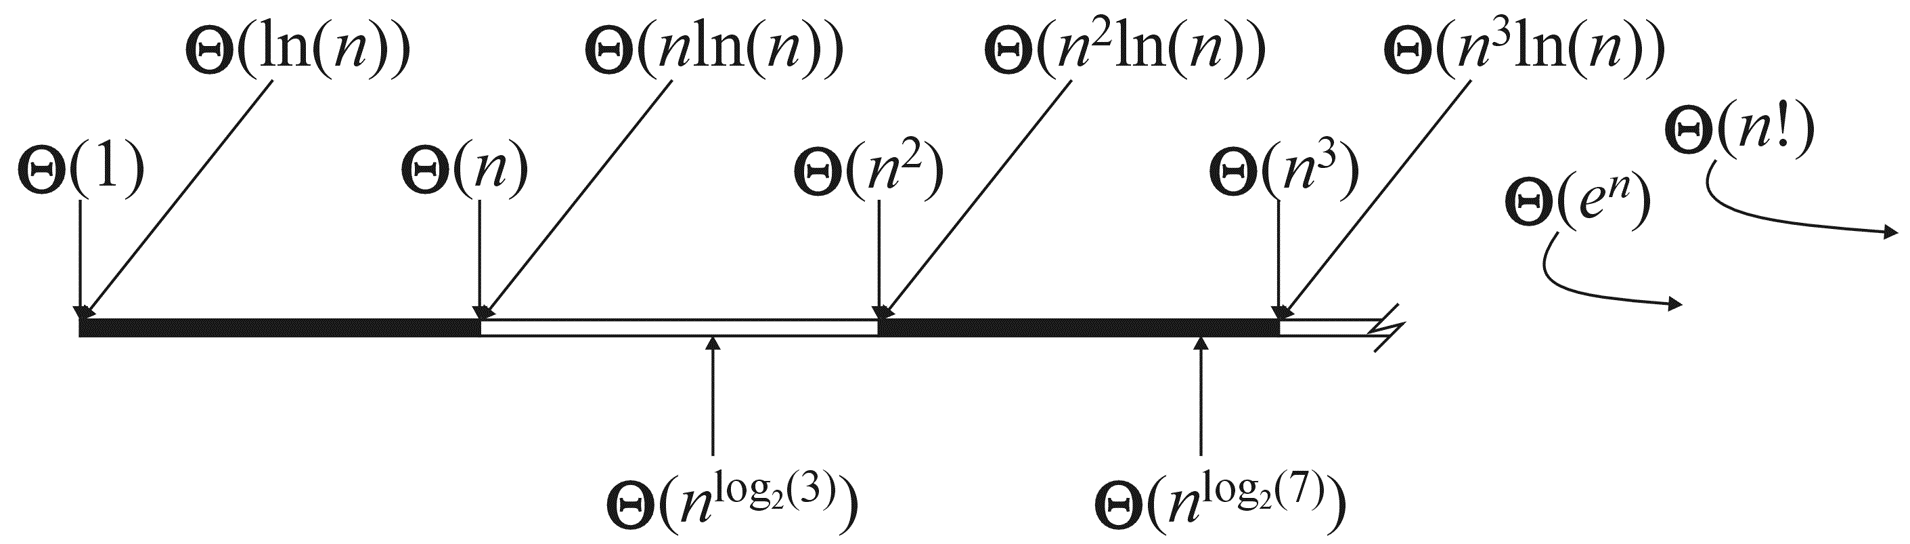
\includegraphics{/media/fika/Documents/Courses/CS240_Algorithm_Design/Midterm Cheatsheet/ThetaOrder.png}
\caption{order}
\end{figure}

\begin{itemize}
\item
  when \(p<q\), \(np = o(\ln(n)n^p)\), but \(\ln(n)n^p = o(n^q)\)
\item
  \((\log n)^k = o(n^ε), ∀k ∈ Z^+, ε ∈ R^+\) 
\item
  \(n! \approx \sqrt{2\pi n}(\frac{n}{e})^n\)

  \begin{itemize}
  \item
    或者表达为:\( \lim_{n\rightarrow \infty} \frac{n!}{\sqrt{2\pi n}(\frac{n}{e})^n}=1\)
  \item
    解释了为什么 \(n!<n^n\), but \(\log(n!)\sim\log(n^n)\)
  \end{itemize}
\end{itemize}

if-else: assume the longest branch runs (worse case complexity)

\hypertarget{recursive-algorithms}{%
\subsection{recursive algorithms}\label{recursive-algorithms}}

\begin{enumerate}
\def\labelenumi{\arabic{enumi}.}
\item
  Find a recurrence relation
\item
  Solve the equation

  \begin{itemize}
  \item
    \textbf{Guess} a solution, then prove it by \textbf{induction}.
  \item
    Substitution: 一直展开式子,直到\(S(n) = S(1)+...\)
  \item
    Recursion tree: 深度和每层上的开销,求和
  \item
    Master theorem

    \begin{itemize}
    \item
      \begin{figure}
      \centering
      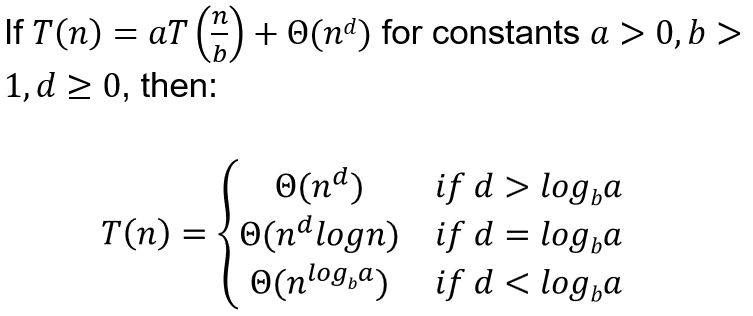
\includegraphics{/media/fika/Documents/Courses/CS240_Algorithm_Design/Midterm Cheatsheet/image-20231101082743665.png}
      \caption{image-20231101082743665}
      \end{figure}
    \item
      可以处理\(T(n) = 3T(n/4)+n\log n\),
      但无法处理\(T(n) = 2T(n/2)+n\log n\)
    \item
      \(T(n)=2T(\sqrt{n})+\Theta(\log n)\): Let
      \(n = 2^m, S(m)=T(2^m)\).
    \end{itemize}
  \end{itemize}
\end{enumerate}

\begin{quote}
\(T(n) = a \cdot T\left(\frac{n}{b}\right) + f(n)\)

其中 \(a \geq 1\),\(b > 1\),\(f(n)\) 是一个正函数,则 \(T(n)\)
的渐进上界可以根据以下三种情况中的一种确定:

\begin{enumerate}
\def\labelenumi{\arabic{enumi}.}
\item
  如果 \(f(n) = O(n^{\log_b a - \epsilon})\) 对某个常数 \(\epsilon > 0\)
  成立,则 \(T(n) = \Theta(n^{\log_b a})\)。
\item
  如果 \(f(n) = \Theta(n^{\log_b a})\),则
  \(T(n) = \Theta(n^{\log_b a} \log n)\)。
\item
  如果 \(f(n) = \Omega(n^{\log_b a + \epsilon})\) 对某个常数
  \(\epsilon > 0\) 成立,且对某个常数 \(c < 1\) 和足够大的 \(n\),有
  \(a \cdot f\left(\frac{n}{b}\right) \leq c \cdot f(n)\),则
  \(T(n) = \Theta(f(n))\)。
\end{enumerate}
\end{quote}

\begin{center}\rule{0.5\linewidth}{0.5pt}\end{center}

\hypertarget{divide-and-conquer}{%
\section{Divide and Conquer}\label{divide-and-conquer}}

\hypertarget{selection}{%
\subsection{Selection}\label{selection}}

\[S(n) \le S(n/5)+S(7n/10)+O(n)\]

\hypertarget{long-multiplication-of-two-integers----karatsuba-s-algorithm}{%
\subsection{Long multiplication of two integers -- Karatsuba' s
algorithm}\label{long-multiplication-of-two-integers----karatsuba-s-algorithm}}

naive \(O(n^2)\)

\begin{figure}
\centering
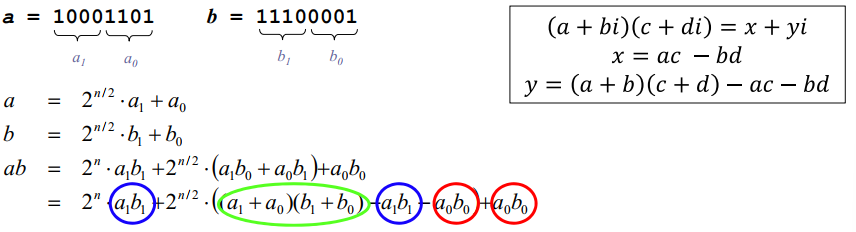
\includegraphics{/media/fika/Documents/Courses/CS240_Algorithm_Design/Midterm Cheatsheet/image-20240229135701150.png}
\caption{image-20240229135701150}
\end{figure}

\begin{itemize}
\item
  It does 3 multiplications of digit numbers instead of 4
\end{itemize}

\[S(n) = 3S(n/2)+O(n)\\
S(n) = \Theta(n^{\log_23}) = O(n^{1.59})< O(n^2)\]

\hypertarget{block-matrix-multiplication}{%
\subsection{Block matrix
multiplication}\label{block-matrix-multiplication}}

naive \(O(n^3)\)

\begin{figure}
\centering
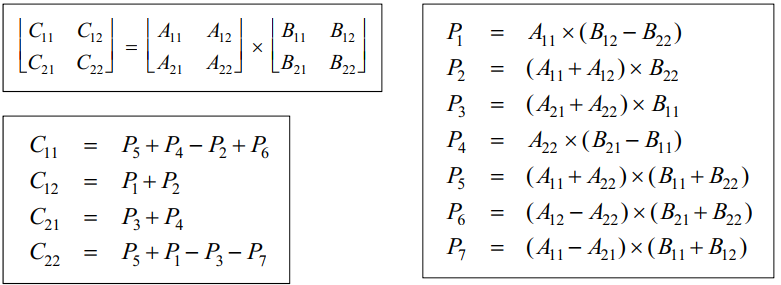
\includegraphics{/media/fika/Documents/Courses/CS240_Algorithm_Design/Midterm Cheatsheet/image-20240229142838424.png}
\caption{image-20240229142838424}
\end{figure}

\[S(n) = 7S(n/2)+O(n^2)\\
S(n) = \Theta(n^{\log_2 7}) = O(n^{2.81})\]

\hypertarget{counting-inversions}{%
\subsection{Counting Inversions}\label{counting-inversions}}

First sort then count

\[S(n) = 2S(n/2) + O(n) \\

S(n) = O(n\log n)\]

\hypertarget{maximum-subarray}{%
\subsection{Maximum Subarray}\label{maximum-subarray}}

\textbf{Goal.} Given array A, find with max \(\sum_{k = i+1}^j A[k]\)

分成两半,要么全左要么全右要么横跨中间\(O(n)\)

\[S(n) = 2S(n/2) + O(n) \\
S(n) = O(n \log n)\]

\hypertarget{closest-point-pair}{%
\subsection{Closest Point Pair}\label{closest-point-pair}}

\end{document}
